\documentclass[11pt]{article}

\usepackage[margin=1.05in]{geometry}
\usepackage{amsmath,amssymb,amsthm}
\usepackage{stmaryrd}
\usepackage{booktabs}
\usepackage{enumitem}
\usepackage{tikz}
\usepackage{listings}
\usepackage[expansion=false]{microtype}
\usepackage{hyperref}
\emergencystretch 2.5em
\usetikzlibrary{arrows.meta,positioning,decorations.pathmorphing,calc}

\hypersetup{colorlinks=true, linkcolor=blue!45!black,
            citecolor=blue!45!black, urlcolor=blue!45!black}

\theoremstyle{plain}
\newtheorem{theorem}{Theorem}[section]
\newtheorem{proposition}[theorem]{Proposition}
\newtheorem{lemma}[theorem]{Lemma}
\newtheorem{corollary}[theorem]{Corollary}
\newtheorem{conjecture}[theorem]{Conjecture}
\theoremstyle{definition}
\newtheorem{definition}[theorem]{Definition}
\newtheorem{observation}[theorem]{Observation}
\newtheorem{construction}[theorem]{Construction}
\theoremstyle{remark}
\newtheorem{remark}[theorem]{Remark}

\newcommand{\Lrn}{\mathcal{L}}
\newcommand{\Nsp}{\mathsf{N}}
\newcommand{\Met}{\mathsf{Met}}
\newcommand{\Src}{\mathsf{Src}}
\newcommand{\Prb}{\mathsf{Prb}}
\newcommand{\Mat}{\mathsf{Mat}}
\newcommand{\Chn}{\mathsf{Chn}}
\newcommand{\sep}[2]{\mathbin{\mid_{#2}^{#1}}}
\newcommand{\fn}{\mathrm{fn}}
\newcommand{\quo}[1]{@#1}
\newcommand{\drop}[1]{*#1}
\newcommand{\AI}{\mathrm{AI}}
\newcommand{\CN}{\mathrm{CN}}
\newcommand{\gen}{\ell}
\newcommand{\Real}{\mathbb{R}}
\newcommand{\Rpos}{\mathbb{R}_{>0}}
\newcommand{\bt}{\beta_1}
\newcommand{\bisim}{\sim}
\newcommand{\bisimn}[1]{\sim_{#1}}
\newcommand{\Ext}{\mathrm{Ext}}
\newcommand{\str}{\mathrm{str}}

\lstset{
  basicstyle=\ttfamily\scriptsize,
  columns=fullflexible,
  breaklines=true,
  showstringspaces=false,
  commentstyle=\color{black!55},
  frame=single,
  framesep=4pt,
  xleftmargin=6pt,
}

\title{\textbf{Scope and Manufacture}\\[4pt]
\large Namespace as the scope of a count, graded copy number, and some
cheap lower bounds on the assembly of a mind}
\author{F1R3FLY.io Research Notes}
\date{2026-08-05}

\begin{document}
\maketitle

\begin{abstract}
\noindent
Assembly theory characterises life by two numbers: an assembly index,
counting the joining steps needed to manufacture an object, and a copy
number, counting how many of that object are present. The first has no
observer and the second has no scope. This note supplies both, using
machinery the companion notes already carry, and finds that once they are
supplied the two numbers stop being independent.

Scope first. A count of copies presupposes a region in which to count, and
if that region is the universe there is no census to take --- not a hard
count but no fact of the matter. The companion notes work throughout in
\emph{namespaces}, and a namespace is exactly a scope. We take one step
past the finite-set-of-channels version: a scope should be a
\emph{predicate} rather than a set, so that it can be finitely described
and yet unbounded in extension. Disjointness of two such predicates is what
makes a composite scope parse uniquely, and so is a feature and not an
obstacle; and with a fixed-point operator, $\mu X.\,\quo{((\phi \lor X)
\mid (\psi \lor X))}$ describes a self-similar scope in a constant number
of symbols. The reflective calculus makes membership in such a scope
decidable by descent, because a name codes a strictly smaller term.

Copy number second. Bisimilarity is the right identity criterion for
copies and is not decidable, so a copy number defined by it is well posed
and uneffective. Relativising to the resolution a learner can afford ---
$n$-step bisimulation, with $n$ bounded by its own assembly index ---
makes the count effective and makes it observer-relative. Coarse observers
\emph{overcount}, geometrically: in a population separating at depth $h$
with branching $b$, an observer of resolution $n$ reports $b^{\,h-n}$
copies where there is one. And in a scope generated by a fixed point the
count is not an integer but a series, one term per stratum; assembly
theory's single number is the flat collapse of that series, licensed only
when the scope has no strata to collapse.

Manufacture third, and lightly. We give six cheap lower bounds on the
assembly index of an ecology-as-mind --- having an inside, owning a
boundary, carrying a germ, resolving at a depth, escaping a basin, and
repairing itself --- and observe that disjointness of the strata is what
lets them be added rather than maximised. None is tight and we do not
argue that tightness is yet the interesting question.

Two things follow that we did not expect. Copies are forced by
repairability and by sampling before they are wanted for statistics, and
the sampling requirement is exponential in depth, so $\CN \gtrsim p^{-h}$
for any ecology that actually uses its architecture: the joint biosignature
acquires a functional form whose base is medium reliability. And the
assembly budget of a multi-skilled mind is dominated by the number of
distinct niches it addresses rather than by the depth of its architecture,
because self-similar architecture is paid for once. A worked
four-skill individual, computed in full, spends $57\%$ of its floor on
content and saves $35\%$ of the unshared budget by sharing its kernel.
\end{abstract}

\tableofcontents

%% ===================================================================
\section{Introduction}\label{sco:S1}

\subsection{The question this note asks}\label{sco:S1.1}

The four notes preceding this one move the unit of learning outward. The
first \cite{scientist} makes an individual mortal scientist out of
cost-accounted rho and a logic of namespaces. The second \cite{game} plays
that individual against an adversary and prices its ladder of hypotheses.
The third \cite{compose} composes learners by parallel composition and
reads the ecological relation between two of them off a grading vector
over typed namespaces. The fourth \cite{engine} gives each community its
own token colour, adjoins engines to convert between them, and finds that
error correction is what decides when a composite may close over its
namespace and become an individual --- at which point the unit has moved
far enough to start again.

That series leaves a natural question unanswered: what does all this
motion \emph{cost}, and in what region is the cost counted? Assembly
theory \cite{assembly,biosig} offers a vocabulary for the first half of
that question. It assigns to an object an \emph{assembly index}: the
minimum number of joining steps needed to build it from elementary
material, where each step may reuse anything already made. And it pairs
that index with a \emph{copy number}, on the thesis that high assembly
index together with high copy number is a biosignature --- that only a
process of selection makes many of a hard-to-make thing.

The pairing is attractive and, we think, correct in outline. Our
complaint is narrower: the two quantities are asymmetrically specified.
The assembly index is a minimum over constructions and so is a property of
the object; whatever else is unclear about it, it does not depend on who
is looking. Copy number does. To count copies of $M$ one must say
\emph{where} to count and \emph{what counts as a copy}, and assembly
theory as it stands says neither.

\subsection{The move, stated once}\label{sco:S1.2}

A namespace is a scope. That is the whole of the observation, and the rest
of this note is what follows from taking it seriously.

If the scope is left implicit, and one tries to make it explicit by
saying ``the universe'', the count does not become large or uncomputable.
It becomes ill-formed: there is no region, no census, no simultaneity in
which to take one, and the quantifier ranges over something that is not a
collection of locations. If instead the scope is a namespace, three things
become available at once. The region is a set of channels, so a count is a
count of channels. The identity criterion is bisimulation, so ``copy''
means behaviourally indistinguishable rather than structurally identical.
And --- this is the part the companion notes make available and assembly
theory cannot --- both the region and the criterion are things a
\emph{budgeted learner} can hold, which means the count acquires the
observer that it needs and that assembly theory forgot to give it.

Once the observer is there, the two numbers couple. The observer's
resolution is bounded by its own manufacture; a coarse observer
overcounts; and the copies that a deep architecture requires are forced by
the fragility of depth. High assembly index and high copy number are not
two independent readings that happen to correlate in living matter. They
are two coordinates on a frontier, and we can write down the frontier.

\subsection{What we claim, and what we do not}\label{sco:S1.3}

We claim: a definition of scope as a predicate rather than a set
(\S\ref{sco:S3}); a proposition that disjointness makes composite scopes
parse uniquely, so that structure is what disjointness buys
(\S\ref{sco:S3.3}); fixed-point scopes and their decidability by descent
(\S\ref{sco:S3.4}); a graded, resolution-indexed copy number
(\S\ref{sco:S4}) with a geometric overcounting law; six cheap lower bounds
on manufacture (\S\ref{sco:S5}); a generator/unfolding distinction with
two ratios (\S\ref{sco:S6}); and a coupling $\CN \gtrsim p^{-h}$ between
the two axes of the biosignature (\S\ref{sco:S7}).

We do not claim that any lower bound in \S\ref{sco:S5} is tight, or even
close. We think they are all loose, in some cases wildly, and we give
them anyway: they are cheap, they are honest, and a floor one can compute
is worth more at this stage than a floor one can defend. The question of
what the \emph{true} minimum manufacture of a mind is seems to us to
require an incompressibility argument of a kind nobody currently knows how
to make in this setting, and we would rather leave the question visible
than paper it over.

We also do not claim that the copy series of \S\ref{sco:S4.3} is the only
possible grading, or that the four-skill composite of \S\ref{sco:S7.5} is
a model of any actual animal. It is an illustration with the numbers
carried through, in the manner of \cite[\S12]{compose}, and its purpose is
to show that the quantities in this note can be computed at all.

%% ===================================================================
\section{What this note carries forward}\label{sco:S2}

Enough to orient; the companion notes carry the detail.

\paragraph{From assembly theory.}
$\AI(M)$ is the minimum number of joining steps from elementary material to
$M$, each step joining two objects already present. $\CN(M)$ counts copies
of $M$ in a sample. The biosignature thesis is that
$\AI(M) \gg 1$ together with $\CN(M) \gg 1$ indicates selection. In the
process setting the index has an exact reading: $\AI(M)$ is the minimum
length of a context-labelled path in the \emph{open} synchronisation tree
from the elementary terms to $M$, because a joining step is precisely a
transition that requires the environment to supply a partner, and those
are the transitions the open tree records.

\paragraph{From \cite{scientist}.}
A computation is ontologically isolated, so its environment is other
computations, and the boundary between them is the \emph{cut}. Across the
cut there are three grades of access: perception (reading structure the
environment has already computed into legible form), interaction
(rendezvous), and reflection (quotation and its inverse). Hypotheses are
formulae of a namespace logic; an assay is a complementary guard pair
whose third outcome is budget-relative refutation. Confinement: an
ultrametric walk of steps all shorter than $2^{-n}$ never leaves the ball
of radius $2^{-n}$, so a purely incremental learner cannot escape its
initial basin.

\paragraph{From \cite{compose}.}
A learner is a distribution over a population together with its resource
reservoirs, and that population \emph{is} a namespace. Learners compose by
parallel composition. Disjointness of namespaces is graded separation at
$k=0$, and the factorisation theorem says disjointness is equivalent to
the absence of a spanning redex and to probabilistic independence of the
composed distributions; the defect of the lax comparison map is the
interaction. Rooting each learner's namespace at its own quotation makes
disjointness a theorem rather than a hope, by freshness-by-quotation.

\paragraph{From \cite{engine}.}
Communication is mediated: a rendezvous is realised by an interposed
process, and this is without loss of generality. Media are processes,
hence nameable, hence form a namespace $\Chn(B)$ one level up the
reflection tower; and \emph{the medium namespace of one level is the
endpoint namespace of the next}, which is the generating step of the
fractal. An individual is a region whose internal media are closed and
whose boundary media are not; perfect closure is death; individuation is a
fixed point and the circularity is the fractality. A percept of
integration depth $d$ survives with probability $p^d$ and costs $d$
metered rendezvous. The price code on the engine graph has total detection
strength $\bt$ by Foster's theorem, so a bridge carries no discipline at
all.

\paragraph{One theorem, used repeatedly.}
No process contains a name that codes itself; a name codes a strictly
smaller term \cite{RHO}. This is what makes the reflection tower
well-founded downwards, what makes freshness by quotation work, and ---
new here --- what makes membership in a fixed-point scope decidable by
descent.

\paragraph{Notation.}
$\quo{P}$ is the name quoting $P$ and $\drop{n}$ the process a name
carries. $\bisim$ is bisimilarity and $\bisimn{n}$ its $n$-step
approximant. $\phi \mid \psi$ is the structural (separating) conjunction
at process level and $\quo{\phi}$ the name predicate satisfied by
$\quo{P}$ when $P \models \phi$. $\sep{\Nsp}{k}$ is graded separation over
a described namespace, as in \cite[\S3]{game}.

%% ===================================================================
\section{Scope}\label{sco:S3}

\subsection{The unbound quantifier}\label{sco:S3.1}

Write the copy number as it is usually given:
\[
  \CN(M) \;=\; \bigl|\{\, x \;:\; x \text{ is a copy of } M \,\}\bigr|.
\]
Two things are unbound. The variable $x$ ranges over --- what? And ``is a
copy of'' is --- which relation?

These are different failures and they fail differently. The second is a
definitional gap: pick a relation and the criterion is fixed, and the
argument is then about whether the relation is the right one. The first is
worse than a gap. If one answers ``the sample'', the number is relative to
a sample that is not part of the theory, so two experimenters with
different jars report different biosignatures for the same chemistry. If
one answers ``the universe'', the number is not merely uncomputable.

\begin{remark}[Universe-as-scope is not a hard count]\label{sco:rem:nocensus}
A count over the universe is ill-formed rather than intractable. It
requires a collection over which to range and a moment at which to range
over it; general covariance denies the second, and the first is not a set
of locations in any sense the theory supplies, since assembly theory has
no notion of location at all. The correct diagnosis is not ``we cannot
evaluate this'' but ``there is nothing here to evaluate''. This matters
because the two diagnoses recommend different repairs. Intractability
recommends approximation; ill-formedness recommends supplying the missing
argument.
\end{remark}

The missing argument is scope, and the companion notes have been working
in one all along without naming it as such.

\subsection{Scope is a predicate, not a set}\label{sco:S3.2}

The obvious repair is to make the scope a finite set of channels. In the
rho calculus a channel is a name $\quo{P}$, so a finite set of channels is
a perfectly good region: a count over it is a count of channels, and every
channel is a location because it is a piece of code at which something
resides.

That repair works and it is too weak. Its weakness is that a finite set
must be given extensionally --- listed --- and a scope worth having is
usually one nobody can list. ``The channels belonging to this organism''
is a scope; so is ``the channels of any learner rooted at $\quo{P}$'', and
so is ``the channels of this organism, and of its organs, and of their
cells, and so on down''. None of these is naturally a list, and the last is
not finite at all.

\begin{definition}[Scope]\label{sco:def:scope}
A \emph{scope} is a name predicate $\Nsp$. The \emph{extension} of a scope
is
\[
  \Ext(\Nsp) \;=\; \{\, n \;:\; n \models \Nsp \,\},
\]
a set of channels, possibly infinite. We write $\quo{\phi}$ for the scope
satisfied by $\quo{P}$ exactly when $P \models \phi$, and read it as
``names of $\phi$-things''.
\end{definition}

\begin{remark}[The extensional version is the flat case]\label{sco:rem:flat}
A finite set of channels $\{c_1,\dots,c_k\}$ is the scope
$\quo{\phi_1} \lor \dots \lor \quo{\phi_k}$ where $\phi_i$ is a
characteristic formula for $\drop{c_i}$. So nothing is lost by the move to
predicates; what is gained is that a scope may now be \emph{finitely
described and unboundedly large}, which is the case every interesting
application is in.
\end{remark}

The gain is not cosmetic. A learner's hypotheses are formulae; a learner's
resources are held at channels; and a learner can only work with a scope
it can \emph{state}. Making scope a predicate puts it in the same
syntactic category as everything else the learner traffics in, which is
what allows the rest of this note to price it.

\subsection{Disjointness is structure}\label{sco:S3.3}

A composite scope should be more tractable than its parts, not less. That
sounds backwards and is not, and the reason is a small proposition about
parsing.

\begin{proposition}[Unique decomposition]\label{sco:prop:parse}
Let $\quo{\phi}$ and $\quo{\psi}$ be scopes with
$\Ext(\quo{\phi}) \cap \Ext(\quo{\psi}) = \emptyset$, and suppose $\phi$
and $\psi$ are separated at grade $0$ in the sense of \cite[\S5]{compose}.
Then every $n \in \Ext(\quo{(\phi \mid \psi)})$ has a unique
decomposition: there are $P, Q$ with $n = \quo{(P \mid Q)}$,
$P \models \phi$, $Q \models \psi$, and $P, Q$ are determined up to
structural congruence.
\end{proposition}

\begin{proof}[Proof sketch]
Existence is the definition of $\mid$ at formula level. For uniqueness,
suppose $n = \quo{(P \mid Q)} = \quo{(P' \mid Q')}$ with $P,P' \models
\phi$ and $Q,Q' \models \psi$. Quotation is injective, so
$P \mid Q \equiv P' \mid Q'$. Grade-$0$ separation says there is no
spanning redex between the parands, so by the factorisation theorem of
\cite[\S5]{compose} the free names of the $\phi$-part and the $\psi$-part
are disjoint. A structural congruence between two parallel compositions
whose parands have disjoint free names permutes parands within each side;
hence $P \equiv P'$ and $Q \equiv Q'$.
\end{proof}

\begin{corollary}[Description is additive under disjointness]
\label{sco:cor:additive}
Under the hypotheses of Proposition~\ref{sco:prop:parse}, the description
length of the composite scope is
$\gen(\quo{(\phi \mid \psi)}) = \gen(\phi) + \gen(\psi) + O(1)$,
and membership testing decomposes: a name is tested by splitting it once
and testing each part against its own predicate.
\end{corollary}

\begin{remark}[Overlap is where you pay, and it is the same payment as before]
\label{sco:rem:overlap}
If the scopes overlap, the split is not unique, and a membership test must
search over splittings rather than perform one. The description of the
composite then does not decompose, and the excess is exactly the defect of
the lax comparison map $\lambda \colon s(\Lrn_1) \otimes s(\Lrn_2) \to
s(\Lrn_1 \mid \Lrn_2)$ of \cite[\S5]{compose}: the interaction between two
learners and the ambiguity in parsing their joint namespace are the same
quantity, seen once dynamically and once syntactically. This is the third
appearance of that pattern in the series, after \cite{compose}'s $\lambda$
and \cite{engine}'s $\theta$.
\end{remark}

So disjointness is not a constraint that composition must work around. It
is the certificate that makes a composite scope \emph{structured}, and
structure is what makes a larger scope cheaper to work in than a smaller
unstructured one. We will use this again in \S\ref{sco:S5.7}, where the
same certificate is what licenses adding lower bounds instead of
maximising them.

\subsection{Fractality by fixed point}\label{sco:S3.4}

Disjoint composition gives wider scopes. It does not by itself give
\emph{deeper} ones --- scopes whose members are themselves composites of
members, all the way down. For that we want a fixed point.

\begin{definition}[Generated scope]\label{sco:def:gen}
Let $\phi, \psi$ be formulae and $X$ a scope variable. The
\emph{generated scope}
\[
  \Nsp \;=\; \mu X.\, \quo{\bigl( (\phi \lor X) \mid (\psi \lor X) \bigr)}
\]
is the least scope $\Nsp$ with
$\Ext(\Nsp) = \Ext\bigl(\quo{((\phi \lor \Nsp) \mid (\psi \lor \Nsp))}\bigr)$,
where in the body a scope variable in a process position is read as
``the drop of a name in $\Ext(X)$''.
\end{definition}

More elaborate generators are available and will be wanted --- one
predicate per skill rather than two, guarded recursion under several
variables, gradings carried through the unfolding --- but this one is
enough to make the points.

\begin{definition}[Stratum]\label{sco:def:stratum}
The \emph{stratum} $\str(n)$ of a name $n \in \Ext(\Nsp)$ is the number of
unfoldings of $\mu X$ needed to derive $n \models \Nsp$. Atoms --- names
of $\phi$-things and $\psi$-things that are not themselves composites ---
have stratum $0$.
\end{definition}

\begin{figure}[t]
\centering
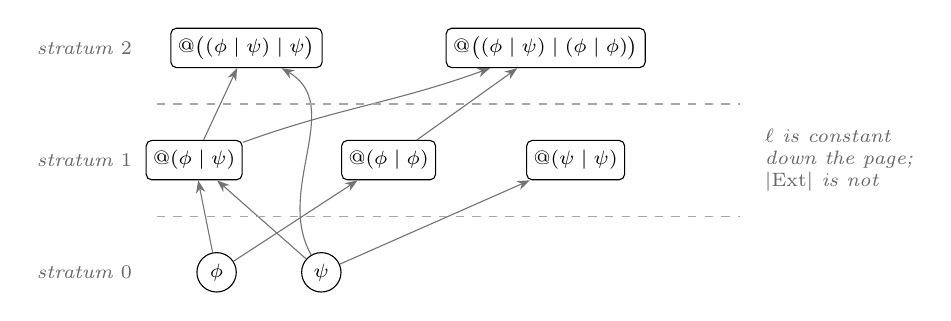
\begin{tikzpicture}[scale=0.95,
  atom/.style={circle,draw,minimum size=5mm,inner sep=0pt,font=\scriptsize},
  comp/.style={rectangle,draw,rounded corners=2pt,minimum height=5mm,
               inner sep=2.5pt,font=\scriptsize},
  lbl/.style={font=\scriptsize\itshape,black!60}]

\node[lbl,anchor=east] at (-0.4,0)   {stratum $0$};
\node[lbl,anchor=east] at (-0.4,1.5) {stratum $1$};
\node[lbl,anchor=east] at (-0.4,3.0) {stratum $2$};

\node[atom] (a) at (0.6,0) {$\phi$};
\node[atom] (b) at (2.0,0) {$\psi$};

\node[comp] (c1) at (0.3,1.5) {$\quo{(\phi\mid\psi)}$};
\node[comp] (c2) at (2.9,1.5) {$\quo{(\phi\mid\phi)}$};
\node[comp] (c3) at (5.4,1.5) {$\quo{(\psi\mid\psi)}$};

\node[comp] (d1) at (1.0,3.0) {$\quo{\bigl((\phi\mid\psi)\mid\psi\bigr)}$};
\node[comp] (d2) at (5.0,3.0) {$\quo{\bigl((\phi\mid\psi)\mid(\phi\mid\phi)\bigr)}$};

\draw[-{Stealth[length=1.6mm]},black!55] (a) -- (c1);
\draw[-{Stealth[length=1.6mm]},black!55] (b) -- (c1);
\draw[-{Stealth[length=1.6mm]},black!55] (a) -- (c2);
\draw[-{Stealth[length=1.6mm]},black!55] (b) -- (c3);
\draw[-{Stealth[length=1.6mm]},black!55] (c1) -- (d1);
\draw[-{Stealth[length=1.6mm]},black!55] (b) to[out=120,in=-30] (d1);
\draw[-{Stealth[length=1.6mm]},black!55] (c1) to[out=20,in=200] (d2);
\draw[-{Stealth[length=1.6mm]},black!55] (c2) -- (d2);

\draw[dashed,black!35] (-0.2,0.75) -- (7.6,0.75);
\draw[dashed,black!35] (-0.2,2.25) -- (7.6,2.25);

\node[lbl,anchor=west,align=left] at (7.8,1.5)
  {$\gen$ is constant\\ down the page;\\ $|\Ext|$ is not};
\end{tikzpicture}
\caption{The extension of a generated scope, stratified. Every name at
stratum $j+1$ quotes a parallel composition of drops of names at stratum
$\le j$, and by Proposition~\ref{sco:prop:parse} that decomposition is
unique. The generator is three symbols wide at every depth; the extension
is not (Table~\ref{sco:tab:growth}).}
\label{sco:fig:strata}
\end{figure}

\begin{table}[t]
\centering
\begin{tabular}{rrr}
\toprule
stratum $\le j$ & $|\Ext_{\le j}(\Nsp)|$ & new at this stratum \\
\midrule
$0$ & $2$      & $2$ \\
$1$ & $5$      & $3$ \\
$2$ & $17$     & $12$ \\
$3$ & $155$    & $138$ \\
$4$ & $12{,}092$ & $11{,}937$ \\
$5$ & $73{,}114{,}280$ & $73{,}102{,}188$ \\
\bottomrule
\end{tabular}
\caption{Extension of the two-atom generator of
Definition~\ref{sco:def:gen}, counted up to structural congruence:
$u_{j+1} = 2 + \binom{u_j+1}{2}$. Computed in
Appendix~\ref{sco:app:num}, block~(1).}
\label{sco:tab:growth}
\end{table}

The extension grows doubly exponentially while the generator does not
grow at all. That gap is the whole point of the construction, and
\S\ref{sco:S6} is about what to make of it. First, though, the property
that makes generated scopes usable rather than merely compact.

\begin{proposition}[Membership is decidable by descent]\label{sco:prop:descent}
Let $\Nsp$ be a generated scope whose atomic predicates $\phi, \psi$ have
decidable satisfaction. Then for any name $n$, the question
$n \models \Nsp$ is decidable.
\end{proposition}

\begin{proof}[Proof sketch]
Test $n$ by unfolding: $n \models \Nsp$ iff either $\drop{n} \models \phi$
or $\drop{n} \models \psi$, or $n = \quo{(P \mid Q)}$ with $\quo{P},
\quo{Q}$ each satisfying $\Nsp$. By
Proposition~\ref{sco:prop:parse} the split is unique, so no search is
needed. The recursive calls are on $\quo{P}$ and $\quo{Q}$, and by the
no-self-code theorem a name codes a strictly smaller term, so
$|P|, |Q| < |P \mid Q|$. The recursion is therefore well-founded on term
size and terminates, with depth bounded by $\str(n) \le |\drop{n}|$.
\end{proof}

\begin{remark}[What is doing the work]\label{sco:rem:whatworks}
Two hypotheses carry this, and neither is decoration. Disjointness makes
the split unique, so the descent is deterministic rather than a search;
that is Proposition~\ref{sco:prop:parse}, and without it the decision
procedure branches over splittings and the complexity is no longer
governed by term size. No-self-code makes the descent well-founded; that
is a property of the reflective calculus specifically, and it is what
prevents a name from being a member of a scope by way of itself. So the
computational coherence of scope here is not merely a matter of
restricting to finite regions. It comes from reflection.
\end{remark}

\begin{remark}[$\mu$, not $\nu$, and this is a claim]\label{sco:rem:munu}
Definition~\ref{sco:def:gen} takes the least fixed point, and the choice is
not innocent. The greatest fixed point admits non-well-founded scopes ---
names whose membership is witnessed only by an infinite descent --- and
Proposition~\ref{sco:prop:descent} does not cover them, because the
argument from no-self-code bounds the descent by term size and a
non-well-founded witness has no such bound. We take the view that the
framework only ever wants $\mu$, and that this is a small result rather
than a convention: \emph{a scope a learner can survey is one whose
membership terminates}, and by \cite[\S6]{scientist} a learner that cannot
terminate a membership test cannot afford the assay that depends on it. A
$\nu$-scope is a scope nothing budgeted can inhabit knowingly. We record
the alternative as an open problem (\S\ref{sco:S9}) rather than as a
settled matter, since a non-well-founded scope is precisely what one would
reach for to model an ecology with no bottom, and we would rather not
foreclose that by fiat.
\end{remark}

\subsection{Scope is an economic quantity}\label{sco:S3.5}

Definition~\ref{sco:def:scope} makes scope statable and
Proposition~\ref{sco:prop:descent} makes membership decidable. Neither
makes a survey affordable, and it is the survey that a copy number
requires.

\begin{definition}[Survey and affordable scope]\label{sco:def:survey}
A \emph{survey} of a scope $\Nsp$ at resolution $n$ is the process of
visiting each $c \in \Ext(\Nsp)$ and deciding $\drop{c} \bisimn{n} P$. Its
cost is one metered rendezvous per visit plus the cost of the depth-$n$
decision, which by \cite[\S4]{game} is $\kappa(n)$ per candidate on the
pricing schedule there. The \emph{affordable scope} of a learner with
budget $\sigma$ is the largest $\Ext_{\le j}(\Nsp)$ whose survey costs at
most $\sigma$.
\end{definition}

\begin{proposition}[Affordable scope is bounded by the profitable radius]
\label{sco:prop:radius}
A learner's affordable scope is contained in the ball of the profitable
radius of \cite[\S7]{engine}. Beyond that radius a channel's traffic
cannot repay the metering and loss of reaching it, so visiting it is a
strictly negative transaction and a learner that performs it is worse off
than one that does not.
\end{proposition}

\begin{remark}[This is what ``computationally coherent'' should mean]
\label{sco:rem:coherent}
Three conditions, and all three are needed. A scope must be
\emph{statable} (a predicate a learner can hold), \emph{decidable} (a
membership test that terminates), and \emph{surveyable} (an extension a
budget can visit). Universe-as-scope fails all three; a finite list of
channels satisfies all three but expresses almost nothing; a generated
scope satisfies the first two by construction and the third stratum by
stratum. So there is a canonical thing to do when a scope is too big:
truncate the unfolding. That is not an approximation to a true count over
a true region. It is the count, taken in the region that exists for this
learner.
\end{remark}

%% ===================================================================
\section{Copy number, graded}\label{sco:S4}

\subsection{Well posed is not effective}\label{sco:S4.1}

With a scope in hand the identity criterion is easy to state. Two
processes are copies when no experiment distinguishes them, and the
relation that says so is bisimilarity. This is the right criterion and not
merely a convenient one: assembly theory's implicit appeal to structural
identity is at once too strict, since two conformers of a molecule are the
same reagent, and too permissive, since two graphs may agree while the
things they denote behave differently under interaction. Behavioural
identity is what a count of copies was always trying to track.

\[
  \CN(P, \Nsp) \;=\; \bigl|\{\, c \in \Ext(\Nsp) \;:\; \drop{c} \bisim P \,\}\bigr|.
\]

This is well posed. It is also not effective: bisimilarity is undecidable
for calculi of this expressiveness \cite{sangiorgi}, so no learner
computes it, and in particular no learner computes this count. The gap is
the same one \cite{scientist} meets in the assay, where a hypothesis that
is true but unaffordable is refuted \emph{relative to a budget}, and the
same remedy applies.

\begin{definition}[Copy number at a resolution]\label{sco:def:cnn}
For a process $P$, a scope $\Nsp$ and $n \in \mathbb{N}$,
\[
  \CN_n(P, \Nsp) \;=\;
  \bigl|\{\, c \in \Ext(\Nsp) \;:\; \drop{c} \bisimn{n} P \,\}\bigr|,
\]
where $\bisimn{n}$ is $n$-step bisimulation. By the Hennessy--Milner
characterisation \cite{HM}, $\drop{c} \bisimn{n} P$ exactly when $\drop{c}$
and $P$ agree on all formulae of modal nesting depth at most $n$.
\end{definition}

\begin{proposition}[Effectivity]\label{sco:prop:effective}
$\CN_n(P,\Nsp)$ is computable for finitely branching processes, any
generated scope $\Nsp$, and any finite $n$, at cost linear in
$|\Ext_{\le j}(\Nsp)|$ and in the depth-$n$ decision procedure.
\end{proposition}

The resolution $n$ is not a free parameter. It is the depth of modal
nesting a learner can afford to evaluate, and that quantity is bounded ---
by integration depth, hence by tower height, hence, if one accepts the
argument of \cite[Ch.~44]{book}, by the learner's own assembly index. So a
count of copies has three arguments and the third belongs to whoever is
counting.

\subsection{The observer enters the count}\label{sco:S4.2}

\begin{proposition}[Coarse resolution overcounts]\label{sco:prop:mono}
For $n' \le n$, $\ \CN_{n'}(P,\Nsp) \;\ge\; \CN_n(P,\Nsp)$, and
$\CN_n \downarrow \CN$ as $n \to \infty$ for image-finite processes.
\end{proposition}

\begin{proof}
$\bisimn{n} \subseteq \bisimn{n'}$ for $n' \le n$, so the counted set
shrinks with $n$; the limit is the standard approximation theorem for
bisimilarity on image-finite processes.
\end{proof}

The direction is worth dwelling on, because it is the opposite of the one
intuition supplies. A weak instrument does not miss copies. It
\emph{manufactures} them, by failing to separate things that differ below
its resolution. And the manufacture is not a small correction.

\begin{proposition}[Geometric overcounting]\label{sco:prop:geom}
Let a population be the leaves of a behaviour tree of depth $h$ and
branching factor $b$, with two members $n$-step bisimilar exactly when
their paths agree for $n$ steps. Then for any member $P$,
\[
  \CN_n(P,\Nsp) \;=\; b^{\,h-n}, \qquad 0 \le n \le h,
\]
so an observer whose resolution falls short of $h$ by $k$ reports
$b^{k}$ times too many copies.
\end{proposition}

\begin{proof}
The members $n$-step bisimilar to $P$ are exactly the leaves of the
depth-$n$ subtree containing $P$, of which there are $b^{h-n}$; at $n=h$
only $P$ itself remains.
\end{proof}

\begin{figure}[t]
\centering
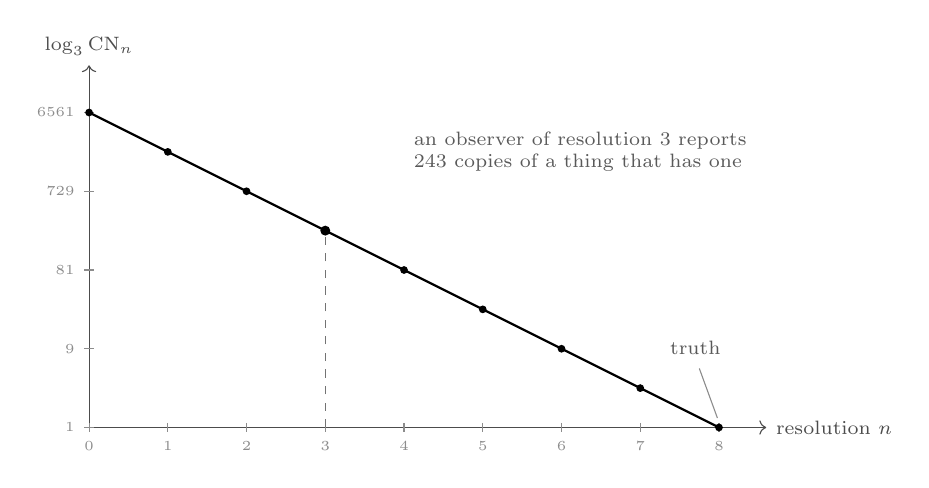
\begin{tikzpicture}[scale=1.0]
  \draw[->,black!70] (0,0) -- (8.6,0) node[right,font=\scriptsize] {resolution $n$};
  \draw[->,black!70] (0,0) -- (0,4.6) node[above,font=\scriptsize] {$\log_3 \CN_n$};
  \foreach \x/\v in {0/0,1/1,2/2,3/3,4/4,5/5,6/6,7/7,8/8}
    \draw[black!45] (\x,0.06) -- (\x,-0.06) node[below,font=\tiny] {\v};
  \foreach \y/\v in {0/1,1/9,2/81,3/729,4/6561}
    \draw[black!45] (0.06,\y) -- (-0.06,\y) node[left,font=\tiny] {\v};

  \draw[thick] (0,4) -- (8,0);
  \foreach \x/\y in {0/4,1/3.5,2/3,3/2.5,4/2,5/1.5,6/1,7/0.5,8/0}
    \fill (\x,\y) circle (1.4pt);

  \draw[dashed,black!55] (3,0) -- (3,2.5);
  \fill[black] (3,2.5) circle (1.8pt);
  \node[font=\scriptsize,anchor=west,black!65,align=left] at (4.0,3.5)
    {an observer of resolution $3$ reports\\ $243$ copies of a thing that has one};
  \draw[black!45] (7.75,0.75) -- (7.98,0.12);
  \node[font=\scriptsize,anchor=south,black!65] at (7.7,0.8) {truth};
\end{tikzpicture}
\caption{Proposition~\ref{sco:prop:geom} for $b=3$, $h=8$; the vertical
axis is logarithmic, so the overcount is the vertical gap to the
right-hand endpoint. Values in Appendix~\ref{sco:app:num}, block~(2).}
\label{sco:fig:overcount}
\end{figure}

\begin{corollary}[A detector has a floor of its own]\label{sco:cor:detector}
To report $\CN$ correctly for a population whose members separate at depth
$h$, an observer must afford resolution $h$, and therefore must itself have
been assembled to a depth supporting modal nesting $h$.
\end{corollary}

\begin{remark}[How far this claim goes, and how far it does not]
\label{sco:rem:notthatfar}
It is tempting to summarise Corollary~\ref{sco:cor:detector} as ``it takes
a mind to find a mind'', and we think that summary is wrong, or at least
much stronger than what is shown. What the observer must match is the
depth at which the \emph{kinds} in the population separate, not the
assembly index of any member of it. Those are very different numbers: in
the worked composite of \S\ref{sco:S7.5} the four kinds separate by depth
$4$ while the individual carrying them has an assembly floor of $28$. A
shallow instrument can therefore certify kind structure it could not
begin to build. What it cannot do is report a copy number that means
anything, and what it will do instead --- silently, with no error signal
--- is report one that is too large by a factor exponential in its
shortfall. That is the useful claim, and it is a claim about
\emph{instruments} rather than about minds.
\end{remark}

\begin{remark}[A false-positive mechanism for the biosignature]
\label{sco:rem:falsepos}
Assembly theory reads $\AI \gg 1$ together with $\CN \gg 1$ as evidence of
selection. Proposition~\ref{sco:prop:geom} says the second conjunct is
inflated by any instrument that cannot resolve the population, and inflated
most where the population is most diverse --- which is to say, exactly
where selection has been most active in generating variants that a coarse
instrument pools. The failure mode is therefore not random noise but a
bias aligned with the signal being sought. We do not know how large the
effect is in the mass-spectrometric practice the theory was designed
around, and we would want that estimated before the criterion is applied
to anything as consequential as an extraterrestrial sample.
\end{remark}

\subsection{The count has a grading it should have kept}\label{sco:S4.3}

In a generated scope there is a second thing wrong with reporting an
integer.

\begin{definition}[Copy series]\label{sco:def:series}
For a generated scope $\Nsp$ with strata $\str$, the \emph{copy series} of
$P$ at resolution $n$ is
\[
  \CN_n^{\bullet}(P,\Nsp) \;=\; \bigl( \CN_n^{(0)}, \CN_n^{(1)},
  \CN_n^{(2)}, \dots \bigr), \qquad
  \CN_n^{(j)} \;=\; \bigl|\{\, c \in \Ext(\Nsp) : \str(c) = j,\
  \drop{c} \bisimn{n} P \,\}\bigr| .
\]
Equivalently, the generating function $\sum_j \CN_n^{(j)} x^j$.
\end{definition}

\begin{remark}[The integer is the flat collapse]\label{sco:rem:collapse}
$\CN_n(P,\Nsp) = \sum_j \CN_n^{(j)}$, so nothing is lost in passing to the
series and a great deal is lost in passing back. The collapse is
legitimate exactly when the scope has one stratum --- when it is a flat
region of like things, which is the situation a jar of reagent
approximates and an organism does not. Assembly theory's copy number is
the flat collapse, and the reason it has felt unproblematic is that the
theory's home application really is a jar.
\end{remark}

\begin{remark}[This agrees with something already in print]
\label{sco:rem:kseq}
\cite[\S8]{engine} concludes, from an entirely different argument about
typed namespaces and the medium tower, that the grading vector $k$ is not
a vector but a \emph{sequence} of vectors, one per stratum. That is the
same observation reached from the composition side rather than the
counting side, and the agreement is some evidence that the stratification
is a feature of the subject rather than of either argument.
\end{remark}

\begin{remark}[What the series is for]\label{sco:rem:seriesfor}
Three uses, in increasing order of speculativeness. First, it distinguishes
architectures that the integer confuses: a colony of $1000$ like cells and
an organism of $1000$ cells in four tissues have the same $\CN$ and
different series. Second, the ratio between consecutive terms is a
branching factor, and \S\ref{sco:S7} argues that this factor is forced from
below by repair and sampling, so the series has a shape one can predict and
check. Third, if the biosignature is to be read off a series rather than a
number, the criterion becomes a statement about the shape --- and ``many
copies at low strata, few at high, with a ratio bounded below by
reliability'' is a much more specific fingerprint than ``$\CN$ is large''.
We do not develop the third here.
\end{remark}

\subsection{A worked series}\label{sco:S4.4}

Take the two-atom generated scope of Definition~\ref{sco:def:gen} and
populate it: let $\phi$-atoms be sources and $\psi$-atoms be foragers, and
let the population instantiate every shape at strata $0$ through $2$ with
multiplicity $12$. Then $|\Ext_{\le 2}| = 17$ shapes
(Table~\ref{sco:tab:growth}), the shapes are distributed $2 : 3 : 12$ over
the strata, and the populated scope has $204$ channels.

Ask for $\CN$ of a stratum-$1$ shape, say $\quo{(\phi \mid \psi)}$. The
truth is $12$. A learner of resolution $2$ separates all three stratum-$1$
shapes and reports $12$. A learner of resolution $1$ separates
$\quo{(\phi\mid\psi)}$ from $\quo{(\phi\mid\phi)}$ but not from
$\quo{(\psi\mid\psi)}$ if the two atoms agree on their first step, and
reports $24$. A learner of resolution $0$ reports $36$, and a learner of
resolution $0$ that also fails to separate strata --- which is what
happens when the instrument counts occurrences rather than channels ---
reports $204$.

The series makes the difference legible where the integer does not:
\[
  \CN_2^{\bullet} = (0,\,12,\,0), \qquad
  \CN_1^{\bullet} = (0,\,24,\,0), \qquad
  \CN_0^{\bullet} = (0,\,36,\,0), \qquad
  \text{flat} = 204 .
\]
Every one of these is a defensible answer to ``how many copies are
there''. Only the first is an answer to ``how many copies are there, at
the resolution at which copies are a kind''.

%% ===================================================================
\section{Manufacture: some cheap lower bounds}\label{sco:S5}

\subsection{What a lower bound would have to be}\label{sco:S5.1}

Upper bounds on what an assembled thing can do are easy in this framework
and we have several. Exhibit an invariant that cannot exceed the assembly
index --- tower height will do --- and then bound capability by the
invariant. Lower bounds run the other way and are much harder, because
$\AI$ is a \emph{minimum} over constructions, so a lower bound is the
claim that no shorter construction exists. That is an incompressibility
statement, and incompressibility statements are notoriously resistant.

There is one tractable route. Find quantities $\iota_1, \dots,
\iota_m$ that are (i) monotone along assembly edges, (ii) forced to a
minimum value by the capability in question, and (iii) witnessed by
\emph{disjoint} sets of edges. Then
\[
  \AI(E) \;\ge\; \sum_i \iota_i(E),
\]
and without (iii) one gets only $\AI(E) \ge \max_i \iota_i(E)$.
Condition (iii) is the hard one in general and, as \S\ref{sco:S5.7}
observes, is exactly what the disjointness of \S\ref{sco:S3.3} certifies
in the cases we care about.

We now give six such quantities. They are all obvious once stated, none
requires an argument longer than a paragraph, and we make no claim that
their sum is anywhere near the truth.

\subsection{Six floors}\label{sco:S5.2}

\begin{table}[h]
\centering
\begin{tabular}{clll}
\toprule
 & capability & floor & from \\
\midrule
L1 & having an inside            & $\AI \ge 1$ & \cite[Def.~5.11]{engine} \\
L2 & owning a boundary           & $\AI \ge 2$ & \cite[Prop.~5.12]{engine} \\
L3 & carrying a germ             & $+1$        & no-self-code \\
L4 & resolving at depth $n$      & $\AI \ge n$ & \cite[Thm.~44.4]{book} \\
L5 & escaping a basin of radius $2^{-n}$ & $\AI \gtrsim n$ & \cite[Prop.~12]{scientist} \\
L6 & repairing itself            & $\AI \ge \bt$ & \cite[Thm.~6.3]{engine} \\
\bottomrule
\end{tabular}
\caption{Cheap floors on the assembly index of an ecology-as-mind. Each is
a paragraph in \S\ref{sco:S5.2}; none is tight.}
\label{sco:tab:floors}
\end{table}

\paragraph{L1: having an inside.}
An ecology-as-mind is a region distinguished from its environment, so
there is at least one medium whose endpoints straddle the boundary. A
medium is a process and must be constructed --- by no-self-code it is not
among the terms it carries --- so its construction is a joining step.
$\AI \ge 1$.

\paragraph{L2: owning a boundary.}
Definition of individual in \cite[\S5.5]{engine}: internal media closed,
boundary media open. That requires the two to be \emph{distinguishable},
hence separately constructed, since a single medium serving both roles
would put the region's interior under external naming and dissolve the
closure that makes repair possible. $\AI \ge 2$. Note that L1 and L2 are
not independent of the requirement that the boundary be porous: by
\cite[Prop.~5.14]{engine} perfect closure is death, so a mind that has
paid for L2 must also have paid for at least one redex pathway across the
boundary, which we fold into L2 rather than counting separately.

\paragraph{L3: carrying a germ.}
The germ of \cite[\S11]{scientist} is a quotation $\quo{P}$, transmissible
and inert until dropped. By no-self-code, $\quo{P}$ is not among the names
occurring in $P$: the germ sits strictly above what it encodes. So the
machinery that manipulates germ material occupies a level of the tower
above the machinery it manipulates, and by the tower-height bound each
level costs at least one edge of a minimum path. Reproduction is $+1$,
unconditionally, over the floor of a thing that does not reproduce.

\paragraph{L4: resolving at depth $n$.}
This one is free: it is the contrapositive of a bound already proved. If
an ecology of assembly index $\AI$ cannot distinguish environments that
are $\AI$-step bisimilar, then an ecology that \emph{does} distinguish
environments differing only at depth $n$ has $\AI \ge n$. Every upper
bound on capability is a lower bound on manufacture, read backwards, and
this is the cleanest instance.

\paragraph{L5: escaping a basin.}
By confinement \cite[Prop.~12]{scientist}, a walk whose steps are all
shorter than $2^{-n}$ never leaves the ball of that radius. Escape
requires a revision move of distance at least $2^{-n}$, which by
\cite[Def.~14]{scientist} means a locus at term-depth at most $n$ and an
operation applied there. Addressing a locus at depth $n$ requires a
one-hole context of that depth, which must be built. So a learner that can
leave its initial basin pays on the order of $n$ steps for the addressing
alone.

\paragraph{L6: repairing itself.}
By Foster's theorem on the engine graph \cite[\S6]{engine}, the total
detection strength of the price code is exactly $\bt$, and an edge that
lies on no cycle has effective resistance $1$ and carries no discipline.
So a region that can detect a single-edge fault has $\bt \ge 1$, and one
that can detect $m$ independent faults has $\bt \ge m$. Each independent
cycle requires an edge that closes it, and those edges are joining steps.
$\AI \ge \bt$.

\subsection{Genetic exploration, and the difference between a learner and a scorer}
\label{sco:S5.3}

L3 and L5 combine into the one bound in this section we find genuinely
interesting, because it separates two things the framework has otherwise
been treating together.

\begin{proposition}[A learner costs strictly more than a scorer]
\label{sco:prop:learner}
Let $S$ be an ecology that evaluates hypotheses drawn from a fixed ball of
radius $2^{-n}$ and never leaves it, and let $L$ be one that can leave. Then
\[
  \AI(L) \;\ge\; \AI(S) + 1 + n^{-},
\]
where the $+1$ is the germ level of L3 and $n^{-}$ is the term-depth of the
shallowest locus whose revision leaves the ball.
\end{proposition}

\begin{proof}[Proof sketch]
By confinement, no sequence of moves available to $S$ leaves the ball, so
whatever $L$ has that $S$ lacks is not a longer run of the same machinery.
By \cite[\S6.5]{scientist} the escape available inside this framework is
recombination, which requires germ material; by L3 germ material costs a
tower level; by L5 the move must address a locus at depth $n^{-}$. The
germ level and the addressing contexts are constructed from different
material --- the first from the learner's own code as quoted, the second
from the term structure being addressed --- so their edges are distinct.
\end{proof}

\begin{remark}[What this says about genetic exploration]\label{sco:rem:genetic}
Read as a design statement rather than a bound: sexual recombination is
not an optimisation of an existing search, it is the purchase of a search
that was not previously available at any price. The confinement result
says an individual cannot get out of its basin by trying harder;
Proposition~\ref{sco:prop:learner} says what getting out costs, and the
cost is structural --- a level of the tower --- rather than metabolic.
That is a satisfying place for the price of sex to sit, because it
explains why the price is paid once, architecturally, rather than
continuously.
\end{remark}

\begin{remark}[The suite of skills does not multiply this]\label{sco:rem:oneg}
A mind with $k$ skills, each realised as an ecology-as-mind, does not pay
L3 $k$ times. The germ is a quotation of the whole individual's code, and
quotation does not distribute over the parts in a way that would require
one germ level per skill. This is the first appearance of the economy that
\S\ref{sco:S6} and \S\ref{sco:S7.5} make quantitative: architecture is
paid for once, content is paid for per skill.
\end{remark}

\subsection{Disjointness is the additivity certificate}\label{sco:S5.7}

\begin{proposition}[Disjoint strata have disjoint witnesses]
\label{sco:prop:disjointedges}
Let an ecology $E$ have strata rooted at pairwise disjoint scopes
$\Nsp_1, \dots, \Nsp_m$ in the sense of \S\ref{sco:S3.3}. Then no single
joining step contributes to two strata, and therefore
$\AI(E) \ge \sum_i \iota(\Nsp_i)$ for any per-stratum floor $\iota$
satisfying (i) and (ii) of \S\ref{sco:S5.1}.
\end{proposition}

\begin{proof}[Proof sketch]
A joining step produces a term $T$; the step contributes to stratum $i$
only if $\quo{T} \in \Ext(\Nsp_i)$. Disjointness of the scopes makes that
membership exclusive, so each step is charged to at most one stratum, and
the per-stratum floors are supported on disjoint edge sets of any
construction path --- in particular of a minimum-length one.
\end{proof}

\begin{remark}[The obligation this discharges]\label{sco:rem:obligation}
The tower-height bound of \cite[Ch.~44]{book} leaves open whether the
joining steps for distinct levels are distinct edges of a single
minimum-length path, noting that if one construction could serve two
levels the count would collapse. Proposition~\ref{sco:prop:disjointedges}
discharges that obligation whenever the levels are rooted at disjoint
scopes --- which, by the rooting discipline of \cite[\S9]{compose}, is
something a designer or a lineage can arrange rather than something that
must be hoped for. The general case, where levels are not disjointly
rooted, remains open, and we suspect it is genuinely harder rather than
merely unwritten.
\end{remark}

\subsection{Why we are stopping here}\label{sco:S5.8}

The sum of Table~\ref{sco:tab:floors} for a reproducing, repairing,
depth-$n$-resolving individual is something like $n + \bt + 4$, and the
worked composite of \S\ref{sco:S7.5} evaluates it at $28$. We believe the
true minimum is very much larger, for the reason
\cite[Rem.~44.2]{book} gives: the assembly index counts everything built,
including redundancy, repair machinery and bulk, while these floors count
only the building that buys a named capability. The ratio between them is
the interesting quantity and we cannot compute it.

We think that is a reasonable place to leave it. A framework earns
attention by making quantities \emph{visible} before it makes them
\emph{sharp}, and a floor that anyone can check and improve is a better
invitation than a theorem that closes the question. The lower bound
problem for minds is, on our reading, at about the stage that the lower
bound problem for circuits was before anyone had a technique: everyone can
see what a bound would have to look like and nobody can produce one.
We would be pleased to be scooped on this.

%% ===================================================================
\section{Generator and unfolding}\label{sco:S6}

Table~\ref{sco:tab:growth} shows a generator of fixed size whose extension
grows doubly exponentially. That gap deserves a name, because the two
quantities on either side of it are measuring different things and the
framework has been conflating them.

\begin{definition}[Generator length]\label{sco:def:genlen}
The \emph{generator length} $\gen(\Nsp)$ of a generated scope is the number
of symbols in the $\mu$-formula defining it, with atomic predicates counted
by their own lengths.
\end{definition}

\begin{proposition}[The chain]\label{sco:prop:chain}
For an ecology $E$ whose namespace is generated by $\Nsp$,
\[
  \gen(\Nsp) \;\le\; h(E) \;\le\; \AI(E)
\]
under the convention that atomic predicates are at least one symbol and
each level of the tower is generated by at least one unfolding.
\end{proposition}

\begin{remark}[Three quantities, three questions]\label{sco:rem:three}
$\gen$ answers ``how long is the description''; $h$ answers ``how many
levels of inside does it have''; $\AI$ answers ``how many steps did it take
to build''. Under $\mu$, $\gen$ is constant while $h$ grows with the
unfolding and $\AI$ grows at least as fast as $h$. Two ratios follow, and
they measure different virtues:
\[
  \frac{h}{\gen} \;=\; \text{how much depth a description buys},
  \qquad
  \frac{h}{\AI} \;=\; \text{architectural efficiency}.
\]
The second is the ratio \cite[Rem.~44.2]{book} proposes as a measure of
how much of an organism's manufacture bought a new inside. The first is
new here, and it is the one that corresponds to something biologists
already measure: a small genome producing a deep organism is a large
$h/\gen$.
\end{remark}

\begin{remark}[The germ is the generator]\label{sco:rem:germgen}
This is not an analogy, and the framework has both objects already. The
germ of \cite[\S11]{scientist} is $\quo{P}$: inert, transmissible,
inspectable, and costing nothing until dropped with $\drop{}$. The
generator of Definition~\ref{sco:def:gen} is a formula: finite,
transmissible, and costing nothing until unfolded. In an ecology whose
namespace is generated, these coincide --- what is inherited is the
generator, and development is the unfolding. The assembly index prices the
unfolding, which is why a genome can be small while its organism is deep,
and why the two numbers were never going to be the same number.
\end{remark}

\begin{remark}[A caution about the direction of the depth bound]
\label{sco:rem:direction}
The bounds of \cite[Ch.~44]{book} are additive: one level, one edge, one
unit of modal depth. That additivity is inherited from the tower argument
and we have no reason to doubt it there. But a lower bound routed through
characteristic formulae rather than through the tower would need to know
how much the modal depth of $\chi_{P \mid Q}$ can exceed those of $\chi_P$
and $\chi_Q$, and if a single joining step can more than increment it then
bounds of that shape degrade from $n$ to $\log n$. We have not needed such
a route here --- all six floors of \S\ref{sco:S5.2} go through structure
rather than through $\chi$ --- but anyone extending this work should check
it before relying on it. We record it in \S\ref{sco:S9}.
\end{remark}

%% ===================================================================
\section{The pressure on copy number}\label{sco:S7}

The two parameters of the biosignature look independent. One is a property
of an object and the other a property of a population, and nothing in
assembly theory relates them except the empirical observation that in
living matter both are large. In this framework they are related, and by
two mechanisms that both push in the same direction: an architecture that
is deep \emph{requires} copies before anybody wants them for statistics.

\subsection{Detection forces copies}\label{sco:S7.1}

By Foster's theorem on the engine graph \cite[\S6]{engine}, the total
detection strength of the price code is $\bt$, distributed over edges by
effective resistance, and an edge on no cycle is undetectable. A region
whose internal media form a tree therefore has no error correction at all:
every fault is silent, and by \cite[Cor.~7.3]{engine} a bridge fails twice,
having neither a cycle to check it nor an owner to repair it.

So repairability requires cycles, and a cycle requires a redundant
pathway, and a redundant pathway between two functional positions is
two copies of a relation where one would carry the traffic. The
requirement recurs per stratum, because each level of the tower has its
own media and its own faults.

\begin{proposition}[Repair floor]\label{sco:prop:repairfloor}
An ecology whose stratum-$j$ media can detect $m_j$ independent single-edge
faults has $\bt^{(j)} \ge m_j$, and therefore carries at least $m_j$ media
in excess of a spanning structure at that stratum.
\end{proposition}

This is a floor on copies of \emph{media}, not of learners, and it is
small --- one per independent fault. The second mechanism is not small.

\subsection{Sampling forces copies, exponentially}\label{sco:S7.2}

By \cite[Prop.~5.18]{engine}, a percept of integration depth $d$ traverses
$d$ hops of internal medium and survives with probability $p^d$. A
hypothesis at that depth needs $m$ independent confirmations before a
learner will fund a revision on it, and confirmations that are attempted
in parallel are attempted by \emph{copies}.

\begin{proposition}[Sampling floor]\label{sco:prop:sampfloor}
To obtain $m$ usable depth-$d$ confirmations per round, an ecology requires
\[
  \CN \;\ge\; \bigl\lceil m\, p^{-d} \bigr\rceil
\]
learners positioned at that depth.
\end{proposition}

\begin{table}[h]
\centering
\begin{tabular}{rrrrrrrrr}
\toprule
$p \backslash d$ & $1$ & $2$ & $3$ & $4$ & $5$ & $6$ & $7$ & $8$ \\
\midrule
$0.99$ & $21$ & $21$ & $21$ & $21$ & $22$ & $22$ & $22$ & $22$ \\
$0.95$ & $22$ & $23$ & $24$ & $25$ & $26$ & $28$ & $29$ & $31$ \\
$0.90$ & $23$ & $25$ & $28$ & $31$ & $34$ & $38$ & $42$ & $47$ \\
$0.80$ & $25$ & $32$ & $40$ & $49$ & $62$ & $77$ & $96$ & $120$ \\
$0.70$ & $29$ & $41$ & $59$ & $84$ & $119$ & $170$ & $243$ & $347$ \\
$0.50$ & $40$ & $80$ & $160$ & $320$ & $640$ & $1280$ & $2560$ & $5120$ \\
\bottomrule
\end{tabular}
\caption{$\lceil m p^{-d}\rceil$ for $m = 20$: copies needed to sustain
$20$ confirmations at integration depth $d$ on media of reliability $p$.
Appendix~\ref{sco:app:num}, block~(3).}
\label{sco:tab:sampling}
\end{table}

\subsection{The two axes are coupled}\label{sco:S7.3}

\begin{proposition}[The frontier]\label{sco:prop:frontier}
An ecology that uses its architecture --- that is, one whose hypotheses
are evaluated at integration depths reaching its tower height $h$ --- has
\[
  \CN \;\gtrsim\; m\, p^{-h},
\]
and since $h \le \AI$, the reachable region of the
$(\AI, \CN)$ plane at reliability $p$ lies above the curve
$\CN = m p^{-\AI}$ only for ecologies that do not use their full depth.
\end{proposition}

\begin{figure}[t]
\centering
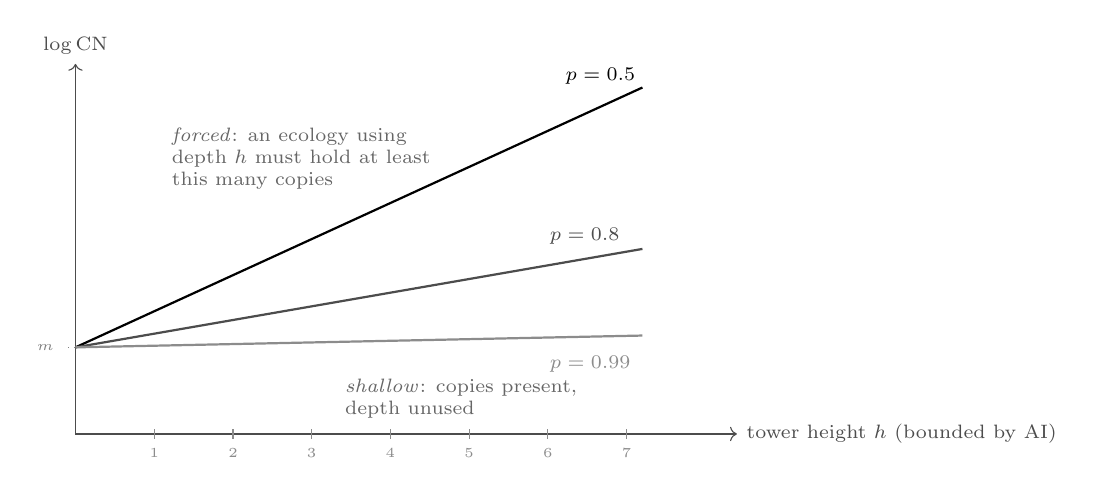
\begin{tikzpicture}[scale=1.0]
  \draw[->,black!70] (0,0) -- (8.4,0) node[right,font=\scriptsize] {tower height $h$ (bounded by $\AI$)};
  \draw[->,black!70] (0,0) -- (0,4.7) node[above,font=\scriptsize] {$\log \CN$};

  \foreach \x/\v in {1/1,2/2,3/3,4/4,5/5,6/6,7/7}
    \draw[black!45] (\x,0.06) -- (\x,-0.06) node[below,font=\tiny] {\v};

  % p = 0.5 frontier : log2 CN = log2 m + h
  \draw[thick] (0,1.1) -- (7.2,4.4);
  \node[font=\scriptsize,anchor=west] at (6.1,4.55) {$p=0.5$};
  % p = 0.8
  \draw[thick,black!70] (0,1.1) -- (7.2,2.35);
  \node[font=\scriptsize,anchor=south west,black!70] at (5.9,2.28) {$p=0.8$};
  % p = 0.99
  \draw[thick,black!45] (0,1.1) -- (7.2,1.25);
  \node[font=\scriptsize,anchor=north west,black!45] at (5.9,1.12) {$p=0.99$};

  \node[font=\scriptsize,anchor=west,black!60,align=left] at (1.1,3.5)
    {\emph{forced}: an ecology using\\ depth $h$ must hold at least\\ this many copies};
  \node[font=\scriptsize,anchor=west,black!60,align=left] at (3.3,0.45)
    {\emph{shallow}: copies present,\\ depth unused};

  \draw[dotted,black!50] (0,1.1) -- (-0.15,1.1) node[left,font=\tiny] {$m$};
\end{tikzpicture}
\caption{Proposition~\ref{sco:prop:frontier}. Each line is
$\log \CN = \log m + h \log(1/p)$: the copy number an ecology must hold to
use a tower of height $h$ on media of reliability $p$. The slope is
set by reliability alone. Assembly theory's joint biosignature is the claim
that living matter sits far to the upper right; this framework says the
two coordinates are not free of each other once the architecture is in
use.}
\label{sco:fig:frontier}
\end{figure}

\begin{remark}[What the biosignature becomes]\label{sco:rem:biosig}
``High $\AI$ and high $\CN$'' is, on this reading, not a conjunction of two
independent findings but a point above a line whose slope is
$\log(1/p)$. The framework accordingly predicts something the bare
conjunction does not: the \emph{ratio} $\log \CN / h$ should cluster near
$\log(1/p)$ for systems that are using their architecture, and fall well
below it for systems that are merely abundant. A crystal is abundant and
shallow; a bacterium is deep and abundant in the proportion its chemistry
can sustain. If the ratio is measurable, this is falsifiable, and it is
falsifiable in a way the conjunction is not.
\end{remark}

\subsection{A prediction about scarcity}\label{sco:S7.4}

Depth is priced exponentially and width linearly. Under a contraction of
resources, a lineage should therefore shed the exponentially priced axis
first.

\begin{remark}[Depth goes before population]\label{sco:rem:shed}
An ecology entering scarcity may reduce $h$ or reduce $\CN$. Reducing $h$
by one releases a factor $p^{-1}$ of the sampling requirement at every
stratum above the cut, together with the media, repair and engine
machinery of the level removed; reducing $\CN$ by one releases one
learner's maintenance. The first is worth vastly more per unit of
structural change. So we expect --- as an empirical matter, and stated as
an expectation rather than a theorem --- that lineages entering sustained
scarcity lose architectural levels before they lose population, and that
the reverse pattern indicates something other than resource pressure.
Regressive evolution in parasites and cave fauna is the obvious place to
look, and the obvious confound is that the same pressure removes the
selective reason for the level as well as the means to pay for it.
\end{remark}

\subsection{A worked composite: four skills, one individual, twelve of them}
\label{sco:S7.5}

We now carry the numbers through a mind whose skills are themselves
ecologies-as-mind, in the manner of \cite[\S12]{compose}. The illustration
is orca-shaped, and the shape is doing no work beyond making the skills
memorable: a hunting skill, a skill for one's place in the pod, a mating
skill, and a skill for rearing calves. Each is a population of mortal
scientists in its own typed namespace with its own token colour; the four
are wired by engines; the whole closes over its namespace and is an
individual; and twelve such individuals form a pod, which is a candidate
individual one stratum up.

\paragraph{The generator.}
The individual's scope is
\[
  \Nsp \;=\; \mu X.\;
  \quo{\bigl( (\phi_{\mathrm{for}} \lor X) \mid
              (\phi_{\mathrm{pod}} \lor X) \mid
              (\phi_{\mathrm{mat}} \lor X) \mid
              (\phi_{\mathrm{rea}} \lor X) \bigr)},
\]
the four-predicate version of Definition~\ref{sco:def:gen}. The four
predicates are pairwise disjoint --- each skill's population is rooted at
its own quotation, per \cite[\S9]{compose} --- so
Proposition~\ref{sco:prop:parse} applies and the scope parses uniquely,
Proposition~\ref{sco:prop:descent} makes membership decidable, and
Proposition~\ref{sco:prop:disjointedges} lets the floors be added.

\paragraph{Depths and populations.}
Each skill sits on media of its own reliability: the pod and rearing
skills run on internal, owned media ($p = 0.99$); hunting reaches across
the boundary into a noisy world ($p=0.95$); mating runs across
\emph{another individual's} boundary and is worst ($p = 0.90$). Optimal
integration depth follows \cite[\S5.5]{engine}, maximising
$Y(d)p^d - cd$ with $Y(d) = 100(1-2^{-d})$ and $c=2$; the sampling floor
follows Proposition~\ref{sco:prop:sampfloor} with $m=20$.

\begin{table}[h]
\centering
\begin{tabular}{lrrrrr}
\toprule
skill & $p$ & $d^\ast$ & net value & $\CN$ floor & separates at \\
\midrule
Forage & $0.95$ & $3$ & $69.0$ & $24$ & $4$ \\
Pod    & $0.99$ & $5$ & $82.1$ & $22$ & $2$ \\
Mate   & $0.90$ & $3$ & $57.8$ & $28$ & $3$ \\
Rear   & $0.99$ & $5$ & $82.1$ & $22$ & $3$ \\
\midrule
       &        &     &        & $96$ & \\
\bottomrule
\end{tabular}
\caption{The four skill-ecologies. ``Separates at'' is the modal depth at
which that skill's learners become distinguishable from the shared kernel
behaviour. Appendix~\ref{sco:app:num}, block~(4).}
\label{sco:tab:skills}
\end{table}

Note which skill is most expensive in copies. It is not the deepest; it is
the one on the worst medium. Mating costs $28$ learners to sustain depth
$3$ while the pod skill costs $22$ to sustain depth $5$, because
reliability enters the floor exponentially and depth only through the
exponent. An architecture is expensive where it is \emph{unreliable},
not where it is deep.

\paragraph{The copy series.}
Twelve individuals, each with $96$ learners in four skill-ecologies:
\[
  \CN^{\bullet}(\text{pod}) \;=\; (1152,\; 48,\; 12,\; 1),
\]
being learners, skill-ecologies, individuals, and the pod itself. The flat
collapse is $1213$, a number that answers no question anyone would ask. It
is worth saying plainly what the series says and the integer does not: the
ratios $1152{:}48{:}12{:}1$ are $24, 4, 12$, and those three numbers are
respectively a sampling floor, a skill count, and a group size --- three
different kinds of fact about the animal, which the collapse blends into
one meaningless total.

\paragraph{The assembly floor.}
Applying Table~\ref{sco:tab:floors} with the additivity of
Proposition~\ref{sco:prop:disjointedges}:

\begin{table}[h]
\centering
\begin{tabular}{lrl}
\toprule
component & steps & from \\
\midrule
kernel: inside, boundary, germ, stack, assay & $5$ & L1--L3, paid once \\
differentia: $d^\ast$ per skill, $3+5+3+5$   & $16$ & L4, L5 \\
wiring: joining four parts, $\lceil \log_2 4\rceil$ & $2$ & \\
engines: four, to close a cycle over four colours & $4$ & L6 \\
closure of the individual's namespace        & $1$ & L2 \\
\midrule
\textbf{floor} & $\mathbf{28}$ & \\
\midrule
same, with no kernel sharing ($5 \times 4$)  & $43$ & \\
\bottomrule
\end{tabular}
\caption{The assembly floor of the four-skill individual.}
\label{sco:tab:floor}
\end{table}

Two numbers to take from this. Sharing the kernel across the four skills
saves $15$ of $43$ steps, or $34.9\%$; and of the $28$ that remain,
$16$ --- $57.1\%$ --- are \emph{content} rather than architecture. The
fractal is cheap and the niches are expensive, which is the quantitative
form of the claim in \S\ref{sco:S5.3}.

\begin{remark}[The economy runs the other way from intuition]
\label{sco:rem:economy}
One expects a mind made of minds to be expensive because it is deep. It is
not: depth is what the fixed point gives away for free, since a generator
that describes one level describes all of them and copies of a made thing
are free in assembly index. What a multi-skilled mind pays for is
\emph{differentiation} --- the distinct predicates, assays and token
colours that make hunting not-mating. Under this accounting an animal's
assembly index tracks the number of distinct niches it addresses far more
closely than the elaborateness of its architecture, and two animals of very
different apparent sophistication addressing the same number of niches
should come out close together.
\end{remark}

\paragraph{Does the whole close?}
By \cite[\S7]{engine} a region may close over its namespace iff its
isoperimetric ratio clears $(\varepsilon\theta/\rho)\,r$. Taking
$\theta = 0.2$, $\rho = 5$, and $\varepsilon = 1-p$ for the relevant
media: the individual, with internal media at $p=0.99$ and two of its four
skills facing outward ($h = 0.5$), has
$\varepsilon\theta/\rho = 4\times 10^{-4}$ and a critical radius
$r^\ast = 1250$ --- it closes with enormous margin. The pod, whose media
run across individual boundaries at $p = 0.90$ and whose isoperimetric
ratio we take as $0.3$, has $\varepsilon\theta/\rho = 4\times 10^{-3}$ and
$r^\ast = 75$. A pod of twelve closes. An aggregation of two hundred does
not.

\begin{remark}[A critical group size, and how much to believe it]
\label{sco:rem:groupsize}
The number $75$ is a computed consequence of parameters we invented, and
nothing in this note determines $\theta$, $\rho$ or the isoperimetric
ratio of a pod. What is not invented is the \emph{shape} of the result:
there is a finite size beyond which a social aggregation cannot close over
its namespace, it scales as $\rho/(\varepsilon\theta)$, and it is set by
the reliability of the media running between individuals rather than by
anything about the individuals. We note without pressing it that the
literature on cohesive group size in social mammals lives in this
neighbourhood, and that the framework predicts the bound should move with
communication reliability rather than with brain size. We would not want
that repeated as a result.
\end{remark}

\paragraph{What a passing instrument sees.}
Finally, the point of \S\ref{sco:S4.2}, made concrete. The four skills'
learners share the kernel and separate at depths $2,3,3,4$. An observer
surveying the pod's namespace at resolution $n$ reports:

\begin{table}[h]
\centering
\small
\begin{tabular}{crrl}
\toprule
resolution $n$ & kinds & largest class & \\
\midrule
$0$ & $1$ & $1152$ & everything is one kind \\
$1$ & $1$ & $1152$ & \\
$2$ & $2$ & $888$ & the pod skill separates \\
$3$ & $4$ & $336$ & mating and rearing separate; foraging is the remainder \\
$\ge 4$ & $4$ & $336$ & truth \\
\bottomrule
\end{tabular}
\caption{An observer's report on the learner stratum, by resolution. Truth
is four kinds, largest class $336$.}
\label{sco:tab:observer}
\end{table}

An instrument at resolution $0$ reports a copy number $3.4$ times the
truth and a monoculture where there are four kinds. At resolution $2$ it
is still wrong by a factor of $2.6$ on the largest class. And note the
small mercy at $n=3$: once every kind but one has been separated, the last
comes free, because what remains in the pool is a kind by elimination. A
survey therefore needs resolution equal to the second-deepest separation,
not the deepest --- a saving of exactly one kind's worth of instrument,
and the only place in this note where the accounting is generous.

%% ===================================================================
\section{What is shown and what is not}\label{sco:S8}

\paragraph{Shown, in the sense that the argument is complete given the
companion notes.}
That a scope may be a predicate rather than a set, and that the
extensional version is the flat special case
(\S\ref{sco:S3.2}). That disjointness makes a composite scope parse
uniquely and its description additive
(Proposition~\ref{sco:prop:parse}, Corollary~\ref{sco:cor:additive}).
That membership in a $\mu$-generated scope is decidable by descent,
because no-self-code bounds the descent by term size
(Proposition~\ref{sco:prop:descent}). That copy number relativised to
resolution is effective, monotone, and geometrically inflated by coarse
instruments (\S\ref{sco:S4.2}). That in a stratified scope the count is a
series and the integer is its collapse (\S\ref{sco:S4.3}). That the six
floors of \S\ref{sco:S5.2} hold, and may be summed when the strata are
disjointly rooted (Proposition~\ref{sco:prop:disjointedges}).

\paragraph{Argued, but resting on a parameter we cannot fix.}
The frontier $\CN \gtrsim m p^{-h}$ (Proposition~\ref{sco:prop:frontier})
depends on $p$, the per-hop reliability of internal media, which is a free
parameter of \cite{engine} and is not measured anywhere. Everything
downstream of it --- the slope in Figure~\ref{sco:fig:frontier}, the
sampling column of Table~\ref{sco:tab:skills}, the critical group size ---
inherits that freedom.

\paragraph{Illustrated only.}
The four-skill composite. Its structure follows the framework; its numbers
follow from parameters chosen to be plausible rather than measured. It
shows that the quantities are computable and roughly what they look like.
It shows nothing about orcas.

\paragraph{Not shown, and we think importantly so.}
That any floor here is tight, or within an order of magnitude of tight.
That the least fixed point is the right one in general
(Remark~\ref{sco:rem:munu}). That the $\CN$ inflation of
Remark~\ref{sco:rem:falsepos} is large in the mass-spectrometric practice
assembly theory actually uses --- we have given a mechanism, not an
estimate. And that any of this is the right way to read Cronin and
Walker's proposal rather than a different proposal wearing its
vocabulary; on that we are content to have made the two readings
comparable.

%% ===================================================================
\section{Open problems}\label{sco:S9}

\begin{enumerate}[leftmargin=*,itemsep=5pt]

\item \textbf{$\nu$-scopes.} Remark~\ref{sco:rem:munu} argues that a
budgeted learner can only inhabit a $\mu$-scope, since membership must
terminate. But an ecology with no bottom --- turtles all the way down ---
is exactly what one would model with $\nu$, and the reflection tower is
bounded below only by no-self-code, which is a fact about names and not
about ecologies. Is there a coherent notion of a scope that is
non-well-founded and yet surveyable stratum by stratum?

\item \textbf{Does one joining step increment modal depth?}
Remark~\ref{sco:rem:direction}. If $\chi_{P\mid Q}$ can have modal depth
much greater than $\max(\chi_P, \chi_Q) + 1$, then bounds routed through
characteristic formulae degrade logarithmically. The tower-routed bounds
are unaffected, but the question should be settled before anyone builds on
the other route.

\item \textbf{The copy series under merger.} \cite[\S8]{engine} shows that
merger sets $\bt = 0$ and destroys factorisation. What does it do to
$\CN^{\bullet}$? Our expectation is that it collapses two adjacent strata
into one, which would make the series a rather direct diagnostic for
whether a composite has merged or merely composed --- and would give
\cite{compose}'s composition/merger distinction an observable signature.

\item \textbf{Affordable scope and the individuation fixed point.}
Definition~\ref{sco:def:survey} makes affordable scope depend on a budget;
\cite[Rem.~5.24]{engine} makes individuation a fixed point. Both are
circular in the same way --- the region determines what can be afforded and
what can be afforded determines the region. Do they have a common solution,
and is the individual the least one?

\item \textbf{The survey is an assay.} A survey visits channels and
decides bisimilarity at depth $n$; that is an experiment, and by
\cite[\S4]{scientist} an experiment has three outcomes, the third being
budget-relative. So a survey has a $\bot$ column, and a copy number is
properly a triple: confirmed copies, confirmed non-copies, and channels
the budget could not settle. What is the right generalisation of
Definition~\ref{sco:def:cnn} that carries the third column, and does the
biosignature criterion survive it?

\item \textbf{Estimating the inflation.} Remark~\ref{sco:rem:falsepos}
gives a mechanism for systematic overcounting in biosignature detection
without giving its size. What is the effective resolution of a mass
spectrometer, expressed as a modal depth over the reaction system it
observes, and how deep do the kinds in a prebiotic soup separate?

\item \textbf{Generator length as a measurable.} $h/\gen$ is proposed in
Remark~\ref{sco:rem:three} as ``how much depth a description buys''. For
organisms, $\gen$ has an obvious candidate proxy and $h$ does not. Is
there a way to estimate the number of levels of \emph{owned} inside an
organism has, independently of anatomy?

\item \textbf{The general additivity question.}
Proposition~\ref{sco:prop:disjointedges} needs disjoint rooting. Ecologies
that arose rather than were designed will have overlapping strata. Is
there a bound on the collapse --- some inclusion--exclusion over the
overlap grades of \cite[\S6]{compose} --- or does the sum fail
catastrophically?

\end{enumerate}

%% ===================================================================
\appendix

\section{Rholang}\label{sco:app:rho}

Two contracts. The first decides membership in a generated scope by
descent, per Proposition~\ref{sco:prop:descent}. The second surveys a
scope and returns a copy series. Both follow the conventions of
\cite[App.~A]{game}: a bare parameter is a name, an \texttt{@}-pattern
binds data, and a channel is passed as \texttt{*c}. Guards marked
\texttt{//!\ ideal} stand for decision procedures we assume rather than
implement.

\begin{lstlisting}
new InScope, Split, Survey, Series, BisimN, Atom in {

  // ---- membership by descent -------------------------------------
  // mu X . @( (phi \/ X) | (psi \/ X) ), presented as a list of
  // atomic predicates and tested by structural descent on the quote.

  contract InScope(@nm, atoms, ret) = {
    // atoms is a list of atomic predicate channels; nm is the name
    // under test.  Stratum 0: the drop satisfies some atom.
    new hit in {
      Atom!(nm, *atoms, *hit) |
      for (@isAtom <- hit) {
        if (isAtom) { ret!(true) }
        else {
          // Stratum j+1: the drop is a parallel composition, and by
          // Prop. "unique decomposition" the split is unique, so no
          // search is required -- one split, two recursive calls.
          new sp in {
            Split!(nm, *sp) |
            for (@p, @q, @ok <- sp) {
              if (not ok) { ret!(false) }
              else {
                new l, r in {
                  InScope!(p, *atoms, *l) |
                  InScope!(q, *atoms, *r) |
                  for (@a <- l & @b <- r) { ret!(a and b) }
                }
              }
            }
          }
        }
      }
    }
  } |

  // Split returns the unique decomposition of a quoted parallel
  // composition.  Termination of the recursion above is exactly the
  // no-self-code theorem: p and q code strictly smaller terms.
  contract Split(@nm, ret) = {
    match *nm {
      { P | Q } => { ret!(@P, @Q, true) }        //! ideal
      _         => { ret!(Nil, Nil, false) }
    }
  } |

  // ---- the survey ------------------------------------------------
  // Visit each channel of the scope, decide n-step bisimilarity with
  // the target, and bin the result by stratum.  One metered
  // rendezvous per visit: this contract is where a copy number is
  // paid for.

  contract Survey(@target, chans, @n, ret) = {
    new tally in {
      tally!({}) |
      for (@c <= chans) {                     // one visit per channel
        new b, s in {
          BisimN!(c, target, n, *b) |         //! ideal, cost kappa(n)
          Stratum!(c, *s) |
          for (@same <- b & @j <- s) {
            for (@acc <- tally) {
              if (same) { tally!(acc.set(j, acc.getOrElse(j,0) + 1)) }
              else      { tally!(acc) }
            }
          }
        }
      } |
      for (@acc <- tally) { ret!(acc) }       // the copy series
    }
  } |

  // The flat collapse, for comparison with the received definition.
  contract Series(@series, ret) = {
    ret!( series.values().fold(0, (a, b) => a + b) )
  }
}
\end{lstlisting}

\noindent
Three things the listing makes visible that the prose does not. The
recursion in \texttt{InScope} has no fixed depth bound in its own code ---
it terminates because of a theorem about the calculus, not because of a
counter. \texttt{Survey} charges once per channel, which is what makes
affordable scope a budget question rather than a definitional one. And
\texttt{Series} exists only to throw information away; it is the received
copy number, written as the lossy projection it is.

\section{Computations}\label{sco:app:num}

All figures in this note come from \texttt{scope.py}, in four blocks.

\paragraph{(1) Extension growth.}
Names of stratum $\le j$ in the two-atom generated scope, counted up to
structural congruence, satisfy $u_0 = 2$ and
$u_{j+1} = 2 + \binom{u_j + 1}{2}$, since the composites at stratum
$\le j+1$ are unordered pairs with repetition drawn from $u_j$ and
parallel composition is commutative. Values in
Table~\ref{sco:tab:growth}: $2, 5, 17, 155, 12\,092, 73\,114\,280$. The
generator is three symbols wide throughout.

\paragraph{(2) Overcounting.}
$\CN_n = b^{h-n}$ for the behaviour-tree population of
Proposition~\ref{sco:prop:geom}. At $b=3$, $h=8$: $6561, 2187, 729, 243,
81, 27, 9, 3, 1$ for $n = 0, \dots, 8$. Plotted as
Figure~\ref{sco:fig:overcount}.

\paragraph{(3) Sampling floor.}
$\lceil m p^{-d} \rceil$ at $m=20$, tabulated in
Table~\ref{sco:tab:sampling} over six reliabilities from $0.99$ down to
$0.50$ and depths $d$ from $1$ to $8$.
The optimal depth column of
Table~\ref{sco:tab:skills} maximises $Y(d)p^d - cd$ with
$Y(d) = 100(1-2^{-d})$, $c=2$, reproducing the $d^\ast$ values of
\cite[App.~B]{engine}: $5$ at $p \ge 0.99$, $3$ at $p \in
\{0.95, 0.90\}$, $2$ at $p = 0.75$.

\paragraph{(4) The composite.}
Four skills with the parameters of Table~\ref{sco:tab:skills}; $96$
learners per individual; twelve individuals; copy series
$(1152, 48, 12, 1)$ against a flat collapse of $1213$; assembly floor $28$
shared against $43$ unshared, a saving of $15$ ($34.9\%$), of which
$16$ of the $28$ ($57.1\%$) is content. Individuation at
$\theta = 0.2$, $\rho = 5$: the individual has
$\varepsilon\theta/\rho = 4\times10^{-4}$ and $r^\ast = 1250$; the pod has
$4\times10^{-3}$ and $r^\ast = 75$. Observer reports by resolution in
Table~\ref{sco:tab:observer}.

%% ===================================================================
\begin{thebibliography}{99}

\bibitem{scientist} F1R3FLY.io, \emph{The Mortal Scientist: learning as
cost-accounted computation in a reflective higher-order calculus},
research note, 2026.

\bibitem{game} F1R3FLY.io, \emph{Learning to Play}, research note, 2026.

\bibitem{compose} F1R3FLY.io, \emph{Composing Learners: populations as
namespaces, parallel composition as the operator, and the ecological
relations that typed overlap generates}, research note, 2026.

\bibitem{engine} F1R3FLY.io, \emph{Engines and Individuals: token
conversion between composed learners, the cycle space as a price code, and
error correction as the criterion of individuation}, research note, 2026.

\bibitem{compaut} F1R3FLY.io, \emph{Compression versus Autonomy: an
error-theoretic account of an architectural crossover common to biology,
silicon, and distributed systems}, research note, 2026.

\bibitem{book} F1R3FLY.io, \emph{Finding Mind}, book manuscript, 2026.
Chapter references are to the draft of 2026-08-05.

\bibitem{RHO} L.~G.~Meredith, M.~Radestock, \emph{A reflective higher-order
calculus}, Electronic Notes in Theoretical Computer Science 141(5):49--67,
2005.

\bibitem{nslogic} L.~G.~Meredith, M.~Radestock, \emph{Namespace logic: a
logic for a reflective higher-order calculus}, in Trustworthy Global
Computing, LNCS 3705, 2005.

\bibitem{HM} M.~Hennessy, R.~Milner, \emph{Algebraic laws for
nondeterminism and concurrency}, Journal of the ACM 32(1):137--161, 1985.

\bibitem{kozen} D.~Kozen, \emph{Results on the propositional
$\mu$-calculus}, Theoretical Computer Science 27(3):333--354, 1983.

\bibitem{caires} L.~Caires, L.~Cardelli, \emph{A spatial logic for
concurrency (part I)}, Information and Computation 186(2):194--235, 2003.

\bibitem{sangiorgi} D.~Sangiorgi, D.~Walker, \emph{The Pi-Calculus: a
theory of mobile processes}, Cambridge University Press, 2001.

\bibitem{assembly} A.~Sharma, D.~Czégel, M.~Lachmann, C.~P.~Kempes,
S.~I.~Walker, L.~Cronin, \emph{Assembly theory explains and quantifies
selection and evolution}, Nature 622:321--328, 2023.

\bibitem{biosig} S.~M.~Marshall et al., \emph{Identifying molecules as
biosignatures with assembly theory and mass spectrometry}, Nature
Communications 12:3033, 2021.

\bibitem{zenil} A.~Uthamacumaran, F.~S.~Abrah\~ao, N.~Kiani, H.~Zenil,
\emph{On the salient limitations of the methods of assembly theory and
their classification of molecular biosignatures}, npj Systems Biology and
Applications 10:82, 2024.

\bibitem{foster} R.~M.~Foster, \emph{The average impedance of an electrical
network}, in Reissner Anniversary Volume, Edwards Brothers, 1949.

\bibitem{smith} E.~Smith, H.~J.~Morowitz, \emph{The Origin and Nature of
Life on Earth}, Cambridge University Press, 2016.

\bibitem{park} D.~Park, \emph{Concurrency and automata on infinite
sequences}, in Theoretical Computer Science, LNCS 104, 1981.

\end{thebibliography}

\end{document}
